\documentclass{scrreprt}

% allow images
\usepackage{graphicx}
% allow chinese
\usepackage{CJK}
% lists
\usepackage{enumitem}
% hyperlinked TOC (note the CJKbookmarks boolean)
\usepackage[CJKbookmarks = true]{hyperref}
% allow figures and tables to hold position
\usepackage{float}
% pretty tables
\usepackage{booktabs}
\usepackage[table]{xcolor}
% symbols
\usepackage{gensymb}
% format headers and footers
\usepackage[automark,headsepline,footsepline,plainfootsepline]{scrlayer-scrpage}
% allow for usage of \Blinddocument to test formatting
\usepackage{mwe}

% options
\graphicspath{{./figures/}}
\definecolor{light-gray}{gray}{0.95}

% define macros
\newcommand{\pchapter}[1]{
	\begingroup\let\clearpage\relax
	\newpage
	\begin{figure}[H]
		
\includegraphics[width=0.25\textwidth]{logo.jpeg}
	\end{figure}
	\chapter{#1}
	\endgroup
}
\newcommand{\modelno}{
	\texttt{FLT\char`_K100\char`_TOF}
}
\newcommand{\upstream}{
	\texttt{https://github.com/diracs-delta/fruition-specs/%
		FLT\char`_K100\char`_TOF}
}
\newcommand{\x}{
	$\times$
}
\newenvironment{ptable}[2][def]
{
	\begin{table}[H]
	\centering
	\rowcolors{1}{white}{light-gray}
	\caption{#1}
	\begin{tabular}{#2}
	\toprule
}
{
	\bottomrule
	\end{tabular}
	\end{table}
}

% define header, title, date
\lohead{
\includegraphics[width=\marginparwidth]{logo.jpeg}}
\title{
	\begin{figure}[H]
		\centering
\includegraphics[width=0.5\textwidth]{logo.jpeg}
	\end{figure}
	\vspace{1cm}
	\flushright
	\Huge{TOF MODULE}\\
	\Huge{HARDWARE SPECIFICATION}\\
	\vspace{2cm}
	\huge{Model No.\ \modelno}\\
	\vspace{2cm}
	\LARGE{Prepared by David Qiu \\ on behalf of FRUITION CO., LTD.}
}
\date{
	Last revision: January 10th, 2020 \\
	Full revision history and latest data sheets are available at \upstream.
}
%%%%%%%%%%%%%%%%%%%%%%%%%%%%%%%%%%%%%%%%%%%%%%%%%%%%%%%%%%%%%%%%%%%%%%%%%%%%%%%%
\begin{document}
\begin{CJK*}{UTF8}{gbsn}
\maketitle
\tableofcontents

\pchapter{Product Overview}
\section{Brief Description}
距离测量传感器,单元测量距离:2.5至10cm

\begin{figure}[H]
\center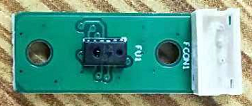
\includegraphics{tof-picture.png}
\caption{产品框图}
\end{figure}

产品描述\ \modelno 是高性能距离测量传感器(TOF)模块,
该产品由以下两个芯片组成,单光子雪崩二极管(SPAD),(红外光电二极管通过红外光带通滤波器)
此模块传感器采用TDC电路系统,覆盖玻璃的串扰特性很好,
传感器自动执行串扰校准,当附着了诸如指纹和污渍时,串扰特性很好,测量精度高,稳定.
该模块传感器具有较强的抗光线干扰能力,物体的反射率、环境温度和工作时间的变化对距离检测影响不大等优点.

\section{产品特性}
\begin{itemize}
	\item 测距传感器采用PSD、红外LED、信号处理电路
	\item 短周期测量(16.5ms)、距离测量范围2.5~10cm
	\item 体积小(21.0\x7.6\x1mm)
	\item 数字I2C输出型
\end{itemize}

\section{应用}
\begin{itemize}
	\item 扫地机器人
	\item 工业机器人
	\item 无人车
\end{itemize}

\section{Figures}
\begin{figure}[H]
\center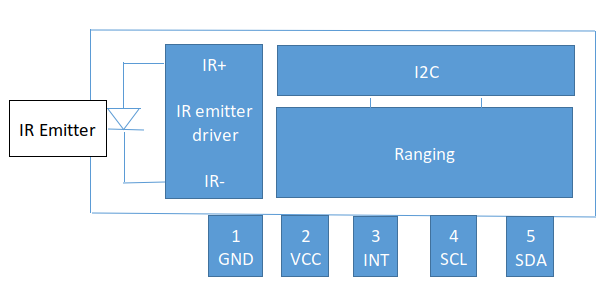
\includegraphics[width=0.9\textwidth]{schematic.png}
\caption{产品框图}
\end{figure}

\begin{figure}[H]
\center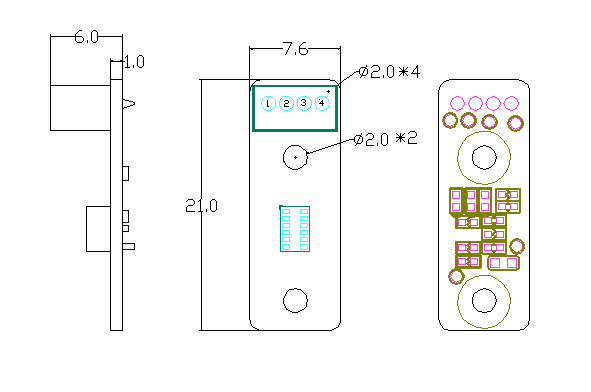
\includegraphics[width=\textwidth]{schematic2.png}
\caption{模组尺寸 (单位: MM)}
\end{figure}

\section{Detailed Specifications}
\begin{ptable}[接口定义]{cccccc}
PIN 1 & GND & --       & PIN 3 & SCL  & CLOCK \\
\midrule
PIN 2 & SDA & DATA BUS & PIN 4 & 3.3V & --    \\
\end{ptable}

\begin{figure}[H]
\center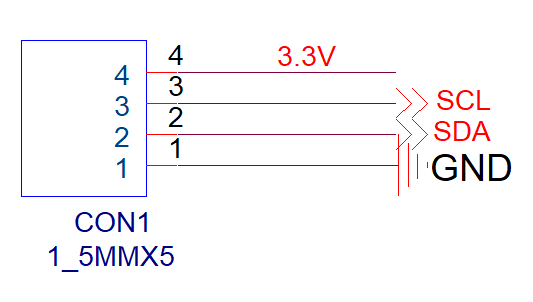
\includegraphics[width=0.5\textwidth]{pins.png}
\caption{接口定义}
\end{figure}

\begin{ptable}[工作条件]{ccccc}
参数   & 符号  & 条件 & 额定值            & 单位        \\
\midrule
工作电压 & VDD & -- & 3.3 $\pm$ 0.15 & V         \\
工作温度 & TA  & -- & $-20$ -- 70    & \degree C \\
\end{ptable}

\begin{ptable}[绝对最大额定值]{ccccc}
参数   & 符号   & 条件  & 额定值             & 单位        \\
供电电压 & VDD  & --  & 0 - 3.8         & V         \\
静电防护 & ESD  & HBM & 2               & kV        \\
储存温度 & TSTG & --  & $-40$ -- $+125$ & \degree C \\
\end{ptable}

\section{串扰校准}
该传感器采用TDC方法,在IC内部生成直方图,并计算出与直方图的距离值。图 \ref{fig:no_cover} 显示了没有盖板玻璃时的直方图,只创建检测到的对象的直方图。图 \ref{fig:cover} 显示了安装盖板玻璃时的直方图。将在检测到的对象旁边创建覆盖玻璃的直方图。在这种情况下,盖板玻璃与被检测对象的直方图重叠,传感器无法计算出正确的距离值。因此,有必要对客户工厂的每个终端进行串扰校准。

\begin{figure}[H]
\center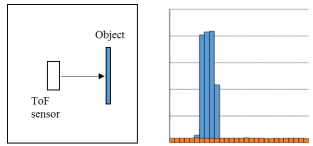
\includegraphics[width=0.8\textwidth]{hist_no_glass.png}
\caption{Histogram without cover glass.}
\label{fig:no_cover}
\end{figure}

\begin{figure}[H]
\center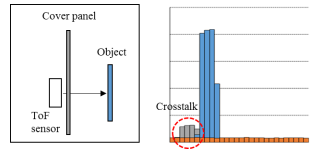
\includegraphics[width=0.8\textwidth]{hist_glass.png}
\caption{Histogram with cover glass.}
\label{fig:cover}
\end{figure}

\begin{figure}[H]
\center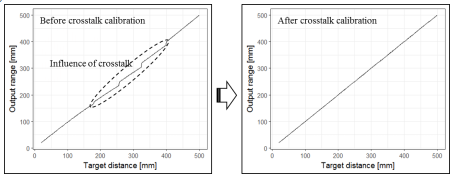
\includegraphics[width=0.9\textwidth]{crosstalk_calib.png}
\caption{Distance response curve before and after crosstalk calibration.}
\end{figure}

\pchapter{串扰校准}
为了提高设计或可靠性,保留在任何时候对本文件所描述的规格、特性、数据、材料、结构和其他内容进行更改的权利。
在本模块应用设计时,请注意以下各点。
对于不符合有关规格表规定的条件,和绝对最高额定值或未满足工作条件的设备不当使用所造成的损害,福临通不承担任何责任。
本产品适用于一般电子设备设计,例如:个人计算机-办公自动化设备-电信设备[终端]-测试和测量设备-工业控制-视听设备-消费电子设备

\end{CJK*}
\end{document}
%%%%%%%%%%%%%%%%%%%%%%%%%%%%%%%%%%%%%%%%%%%%%%%%%%%%%%%%%%%%%%%%%%%%%%%%%%%%%%%%
